\chapter{Comunicando Paramics con OMNeT++ mediante TraCI}
\section{Diseño Arquitectural}\label{sec:architecture}

El software desarrollado consiste en un \emph{plugin} que extiende la funcionalidad de Paramics, agregándole la capacidad de comportarse como un servidor TraCI. Específicamente, el \emph{plugin} consiste en una implementación parcial de un servidor TraCI, el cual se ejecuta en un \emph{thread} paralelo a Paramics; este se encuentra a su vez simulando en modo discreto, esperando instrucciones para avanzar la simulación. La comunicación entre ambos se efectúa a través de la API de extensión de Paramics.

La figura \ref{fig:ptraci_arch} ilustra esta arquitectura. A pesar de que se encuentra implementado como un \emph{plugin} de Paramics, el servidor TraCI es prácticamente un programa independiente, y su interacción con el simulador de transporte se limita a un conjunto acotado de llamados a su API.

\begin{figure}[h]
    \centering
    \begin{sequencediagram}
    \newthread{D}{OMNeT++}{}
    \newinst[1]{A}{VEINS}{}
    \newinst[3]{B}{Plugin (TraCIServer)}{}
    \newthread[2]{C}{Paramics}{}
    
    \begin{messcall}{C}{run()}{B}
        \postlevel
        \begin{call}{B}{waitForCommands()}{B}{}
        \end{call}
    \end{messcall}
    
    \begin{call}{D}{Solicitud}{A}{Resultado}
    
        \begin{call}{A}{Comando TraCI}{B}{Respuesta TraCI}
            \begin{call}{B}{parseCommand()}{B}{sendResponse()}
                \postlevel
                \begin{call}{B}{API Paramics}{C}{Datos}
                \end{call}
                \postlevel
            \end{call}
        \end{call}
    \end{call}
\end{sequencediagram}
    \caption{Arquitectura del Framework}
    \label{fig:ptraci_arch}
\end{figure}

En términos de implementación, el código del \emph{plugin} se separó en una serie de módulos lógicos que encapsulan y abstraen cada uno una categoría de funcionalidades de la interfaz con TraCI. De esta manera, se logró una separación lógica de las funcionalidades implementadas, y se simplifican futuras extensiones al código. 

\begin{figure}
    \dirtree{%
        .1 src/.
        .2 plugin.c\DTcomment{Archivo de inicio del \emph{plugin}}.
        .2 TraCIAPI/\DTcomment{Implementación de la API}.
        .3 Constants.h\DTcomment{Constantes utilizadas en el sistema}.
        .3 Exceptions.h\DTcomment{Excepciones propias del framework}.
        .3 Network.\{cpp/h\}\DTcomment{Métodos de interacción con la red vehicular}.
        .3 Simulation.\{cpp/h\}\DTcomment{Métodos de interacción con la simulación vehicular}.
        .3 Subscriptions.\{cpp/h\}\DTcomment{Suscripciones TraCI}.
        .3 TraCIServer.\{cpp/h\}\DTcomment{Módulo principal, manejo de conexiones TraCI}.
        .3 Triggers.\{cpp/h\}\DTcomment{Operaciones disparadas (temporales o situacionales)}.
        .3 Utils.\{cpp/h\}\DTcomment{Funciones auxiliares y de conveniencia}.
        .3 VehicleManager.\{cpp/h\}\DTcomment{Métodos de interacción con vehículos}.
        .2 shawn/\DTcomment{Archivos externos}.
        .3 socket.\{cpp/h\}\DTcomment{Manejo simplificado de \emph{sockets} TCP}.
        .3 storage.\{cpp/h\}\DTcomment{Manejo simplificado de paquetes de datos}.
    }
    \caption{Estructura de archivos del código fuente del framework.}
    \label{fig:dirtree}
\end{figure}

Describir separación de archivos, namespaces.

\section{Funcionalidad Implementada}

Como se detalló en la sección \ref{sec:traci}, el protocolo TraCI define más de 30 comandos distintos, cada uno con una gran cantidad de variables y parámetros asociados. Implementar esta gran cantidad de funcionalidades no hubiese sido factible, por lo que se escogió un subconjunto acotado de éstas a implementar, considerando en específico aquellos comandos esenciales para simulaciones de ITS.

\subsection{Comandos Implementados}

\subsubsection{Comandos de Control de Simulación}

Se implementaron los tres comandos principales de esta categoría:
\begin{enumerate}
    \item \texttt{0x00} Obtención de Versión
    \item \texttt{0x02} Avance de Simulación
    \item \texttt{0xff} Cierre de Conexión
\end{enumerate}

\begin{enumerate}
    \item test
    \begin{multicols}{2}
        \begin{enumerate}
            \item 1
            \item 2
        \end{enumerate}
    \end{multicols}
\end{enumerate}

\section{Módulos Principales}
\subsection{plugin.c}

Si bien en estricto rigor no es un módulo del \emph{framework}, merece ser mencionado al ser el archivo principal del \emph{plugin} desarrollado. En este archivo se definen las funciones de extensión (prefijo \texttt{QPX}, ver sección \ref{sec:paramics_api}) a ser invocadas por Paramics al inicializar el \emph{plugin}. A continuación se describirán brevemente las más importantes de estas funciones, mientras que el archivo \texttt{plugin.c} puede estudiarse en su totalidad en el código \ref{code:pluginc} en los anexos.

\subsubsection{\texttt{void qpx\_NET\_postOpen(void)}}\label{sec:qpx_postopen}

Invocada inmediatamente luego de que Paramics carga la red y el \emph{plugin}, esta función cambia el modo de ejecución de Paramics a su modo discreto e inicializa el servidor TraCI. Para esto, crea un \emph{thread} donde corre una función auxiliar \texttt{runner\_fn()}, la cual se encarga de:

\begin{enumerate}
    \item Obtener el puerto en el cual esperar conexiones entrantes desde los parámetros de ejecución de Paramics. De no haberse especificado puerto, utiliza uno por defecto.
    \item Inicializar un objeto \texttt{TraCIServer} (ver sección \ref{sec:traciserver}) encargado de las conexiones entrantes en el puerto anteriormente definido.
\end{enumerate}

\subsubsection{\texttt{void qpx\_VHC\_release(VEHICLE* vehicle)}}

Función invocada por Paramics cada vez que un vehículo es liberado a la red de transporte. Simplemente se encarga de notificar al \texttt{VehicleManager} (ver sección \ref{sec:vehiclemanager}) para su inclusión en el modelo interno del \emph{plugin}.

\subsubsection{\texttt{void qpx\_VHC\_arrive(VEHICLE* vehicle, LINK* link, ZONE* zone)}}

Invocada cuando un vehículo alcanza su destino final, esta función notifica al \texttt{VehicleManager} para eliminar el vehículo en cuestión de la representación interna.

\subsection{TraCIServer}\label{sec:traciserver}

Implementa el funcionamiento base del servidor TraCI. Es el primer módulo como tal en inicializarse, y tiene como funciones:

\begin{enumerate}
    \item Asociarse a un \emph{socket} TCP, y esperar una conexión de un cliente TraCI.
    \item Mientras exista una conexión abierta, recibir e interpretar comandos TraCI entrantes.
    \begin{itemize}
        \item En el caso de los comandos de obtención de versión y cierre de la conexión, estos son ejecutados por el módulo mismo.
        \item El comando de avance de simulación es ejecutado parcialmente por este módulo y el módulo \texttt{Simulation} (ver sección \ref{sec:simulation}). Específicamente, se delega el avance del estado de la simulación a \texttt{Simulation}, luego del cual se realiza la evaluación de las suscripciones en \texttt{TraCIServer}.
        \item Demás comandos son delegados a los módulos pertinentes.
    \end{itemize}
    \item Enviar mensajes de estado y respuesta a comandos TraCI.
    \item Al recibir un comando de cierre, finalizar la simulación y cerrar el \emph{socket}.
\end{enumerate}

El módulo en cuestión se implementó como una clase de C++ en los archivos \texttt{src/TraCIAPI/TraCIServer.h} y \texttt{src/TraCIAPI/TraCIServer.cpp}, y se instancia en el archivo \texttt{plugin.c}. Se implementó considerando que se ejecutaría en un \emph{thread} paralelo al principal de Paramics, y por lo tanto incluye elementos de sincronización.

Cabe destacar que para facilitar el uso de \emph{sockets} y la obtención y envío de datos a través de éstos, se utilizaron las clases \texttt{tcpip::Socket} y \texttt{tcpip::Storage}, definidas en los archivos \texttt{src/shawn/socket.\{cpp/h\}} y \texttt{src/shawn/storage.\{cpp/h\}}. \texttt{tcpip::Socket} abstrae el funcionamiento de un \textit{socket} TCP, y provee métodos de conveniencia que permiten leer y escribir mensajes TraCI completos como objetos \texttt{tcpip::Storage}. Estos a su vez proveen métodos para escribir y leer todo tipo de variables en dichos mensajes, sin la necesidad de hacer la conversión manual a bytes.

Estos archivos no fueron desarrollados por el memorista, sino que fueron obtenidos desde el código fuente de SUMO \footnote{Fuente SUMO: \url{https://github.com/planetsumo/sumo/tree/master/sumo/src/foreign/tcpip}. Debe notarse que, a su vez, los creadores de SUMO originalmente obtuvieron dichos archivos del código fuente del simulador de eventos discretos para redes de sensores \emph{SHAWN} \cite{kroller2005shawn}. Su fuente original se encuentra en \url{https://github.com/itm/shawn/tree/master/src/apps/tcpip}}, distribuidos bajo una licencia BSD\footnote{Licencia clases \texttt{tcpip::Socket} y \texttt{tcpip::Storage}: \url{http://sumo.dlr.de/wiki/Libraries_Licenses\#tcpip_-_TCP.2FIP_Socket_Class_to_communicate_with_other_programs}}.

A continuación se detalla la implementación de las funcionalidades anteriormente mencionadas.

\subsubsection{Inicio de conexión TraCI}

Como se mencionó en la sección \ref{sec:qpx_postopen}, al iniciarse el \emph{plugin} se crea un nuevo \emph{thread}, en el cual se instancia un objeto de la clase \texttt{TraCIServer}, al cual se le invoca su método \texttt{run()} (código \ref{cod:traciserver_run}).

\lstinputlisting[float=t, style=CPP, label={cod:traciserver_run}, caption={Rutina de inicio de conexión.}]{codigo/traciserver_run.cpp}
%\minipagelisting{codigo/traciserver_run.cpp}{Rutina de inicio de conexión.}{cod:traciserver_run}

Este método es simple: imprime información pertinente sobre el \emph{plugin} en la ventana de información de Paramics, y luego procede a bloquear el \emph{thread} mientras espera una conexión entrante en el \emph{socket}. Al recibirla, resume la ejecución y realiza un llamado al método \texttt{waitForCommands()} para comenzar a recibir e interpretar comandos TraCI.

\subsubsection{Recepción e Interpretación de Comandos Entrantes}

El método \texttt{waitForCommands()}, presentado en el código \ref{cod:traciserver_waitforcommands}, se encarga de recibir mensajes TraCI entrantes y separar los comandos para su posterior interpretación.

El código inicia un \emph{loop} dentro del cual monitorea el \emph{socket}. Al recibir datos entrantes, el \emph{socket} retorna un objeto \texttt{tcpip::Storage} con el mensaje completo. Luego, en un \emph{loop} adicional, este mensaje se separa en sus comandos TraCI constituyentes, copiando la información perteneciente a cada comando en otro objeto \texttt{tcpip::Storage} temporal. Este objeto se entrega como parámetro al método \texttt{parseCommand()} para la interpretación del comando, luego de lo cual se limpia y se vuelve a utilizar para el siguiente comando.

Finalmente, interpretados todos los comandos, se envía la respuesta al cliente a través del mismo \emph{socket} y se limpian los objetos \texttt{tcpip::Storage} para su reutilización en una nueva iteración del \emph{loop}.

\lstinputlisting[style=CPP, label={cod:traciserver_waitforcommands}, caption={Recepción de mensajes desde el \emph{socket} TCP.}]{codigo/traciserver_waitforcommands.cpp}
%\minipagelisting{codigo/traciserver_waitforcommands.cpp}{Recepción de mensajes desde el \emph{socket} TCP.}{cod:traciserver_waitforcommands}

Como se mencionó anteriormente, la interpretación de los comandos se lleva a cabo en el método \texttt{parseCommand()}, el cual recibe un único comando encapsulado en un objeto \texttt{tcpip::Storage}. Este método tiene una única misión; interpretar el identificador del comando recibido y delegar su ejecución al método correspondiente de la clase \texttt{TraCIServer}. Su implementación es simple, aunque un poco tediosa, y su esqueleto puede observarse en el código \ref{cod:traciserver_parsecommand}. En específico, el código del método se puede dividir en dos ramas de ejecución; en caso de comando de suscripción (cuyos identificadores se encuentran todos en el rango $[\texttt{0xd0}, \texttt{0xdb}]$) se extraen los parámetros de la suscripción y se invoca el método \texttt{addSubscription()} para la subsecuente validación y activación de ésta. Por el contrario, en case de recibir un comando con identificador fuera de dicho rango, se procede a verificar su tipo mediante un \emph{switch}. Cada caso se relaciona con un comando y método específico a invocar, y en caso de no encontrarse el identificador en cuestión se notifica al cliente que el comando deseado no está implementado.

\lstinputlisting[style=CPP, label={cod:traciserver_parsecommand}, caption={Esqueleto de \texttt{parseCommand()}}]{codigo/traciserver_parsecommand.cpp}

Se definieron una serie de comandos en \texttt{TraCIServer} encargados de obtener variables de la simulación o modificar el estado de esta. El funcionamiento de estos es idéntico en todos los casos (a excepción de \texttt{cmdGetPolygonVar()}), y se limita al siguiente procedimiento (ver ejemplo en el código \ref{cod:traciserver_cmdgetvhcvar}):

\begin{enumerate}
    \item Obtener el valor desde el módulo apropiado (por ejemplo, \texttt{VehicleManager} para variables de vehículos, \texttt{Simulation} para variables de la simulación, etc.).
    \item En caso de error en la obtención de los datos (variable no implementada, objeto no existente, etc.), atrapar el error y determinar el curso de acción apropiado (por ejemplo, notificar al cliente).
    \item Finalmente, enviar un mensaje de estado de la solicitud y, en caso de éxito, el valor de la variable, al cliente.
\end{enumerate}

\lstinputlisting[style=CPP, label={cod:traciserver_cmdgetvhcvar}, caption={Ejemplo de método de obtención y empaquetado de variables en \texttt{TraCIServer}}]{codigo/cmdGetVhcVar.cpp}

El caso de \texttt{cmdGetPolygonVar()} es especial. En TraCI, un polígono representa un edificio o una estructura presente en las cercanías de la simulación vehicular, la cual puede interferir con el modelo de comunicación inalámbrica en OMNeT++. Sin embargo, el modelador de Paramics no maneja elementos externos a la simulación de transporte, por lo que se decidió, en el caso de comandos de obtención de variables relacionadas, simplemente reportar que no existen polígonos en la simulación para simplificar la integración.

%Nótese que no se implementó el protocolo en su totalidad, sino únicamente aquellas funcionalidades críticas para su uso práctico en simulaciones de mediana complejidad.


\subsubsection{Avance de Simulación y Evaluación de Suscripciones}\label{sec:traciserver_simstep}

En caso de recibir un comando de avance de simulación, \texttt{TraCIServer} ejecuta su método \texttt{cmdSimStep()}, dentro del cual extrae los parámetros del comando y delega la ejecución de dicho avance al módulo \texttt{Simulation}. Sin embargo, al terminar este procedimiento, se realiza la evaluación de las suscripciones activas en \texttt{TraCIServer}, mediante el método \texttt{processSubscriptions()}.

Como se detalló en la sección \ref{sec:traci}, el protocolo TraCI define 12 tipos de suscripciones a variables de objeto, las cuales comparten todas una estructura idéntica. Cada suscripción se caracteriza por su identificador de tipo y sus parámetros: tiempo de inicio, tiempo de fin, identificador del objeto y las variables a las cuales el cliente se ha suscrito. En la práctica, lo único que diferencia a las suscripciones entre sí son las categorías de objetos a las cuales están asociadas, y por ende, cómo obtener esos datos desde la implementación interna del \emph{plugin}. A raíz de esto, se decidió implementar un árbol de clases de C++ para representar las suscripciones en memoria (declarada e implementada en los archivos \texttt{src/TraCIAPI/Subscriptions.h} y \texttt{src/TraCIAPI/Subscriptions.cpp} respectivamente).

La raíz de éste árbol, la clase \texttt{VariableSuscription}, implementa la funcionalidad completa de evaluación y actualización de una suscripción en los métodos \texttt{handleSubscription()} y \texttt{updateSubscription()} (implementación completa de estos métodos en \ref{code:variablesubscription_main}), abstrayendo la obtención de datos específicos a cada tipo en los métodos \texttt{getObjectVariable()} y \texttt{getResponseCode()}. Estos métodos son \emph{virtuales} en la clase base, y son implementados por las clases derivadas, de manera que \texttt{TraCIServer} sólo necesita mantener un vector de variables del tipo base, las cuales se evalúan de manera polimórfica.

\begin{figure}
    \centering
    \begin{tikzpicture}% [ show background grid ]
    \begin{class}[text width=8cm]{VariableSubscription}{0 ,0}
        \operation{uint8\_t handleSubscription(\dots) \{\dots\}}
        \operation{uint8\_t updateSubscription(\dots) \{\dots\}}
        \operation[0]{virtual void getObjectVariable(\dots);}
        \operation[0]{virtual uint8\_t getResponseCode();}
    \end{class}
    
    \begin{class}[text width=7cm]{VehicleVariableSubscription}{4 ,-4}
        \inherit{VariableSubscription}
        \operation{void getObjectVariable(\dots) \{\dots\}}
        \operation{uint8\_t getResponseCode() \{\dots\}}
    \end{class}
    
    \begin{class}[text width=7cm]{SimulationVariableSubscription}{-4 ,-4}
        \inherit{VariableSubscription}
        \operation{void getObjectVariable(\dots) \{\dots\}}
        \operation{uint8\_t getResponseCode() \{\dots\}}
    \end{class}
\end{tikzpicture}
    \caption{Diagrama de herencia, \texttt{VariableSubscription}}
    \label{fig:cd_variablesub}
\end{figure}

En términos más simples, lo único que debe implementar una clase derivada de \texttt{VariableSubscription} para definir un nuevo tipo de suscripción son versiones propias de los métodos \texttt{getObjectVariable()} y \texttt{getResponseCode()}, ya que todo la demás funcionalidad de evaluación de suscripciones está ya implementada en la clase base. 
%Para dar un ejemplo, para suscripciones de variables de vehículos, estos métodos se ven así:

%\lstinputlisting[style=CPP, label={cod:vehiclesub}, caption={Ejemplo de métodos extendidos en \texttt{VehicleVariableSubscription}}]{codigo/vehiclesub.cpp}
%\minipagelisting{codigo/vehiclesub.cpp}{Ejemplo de métodos extendidos en \emph{VehicleVariableSubscription}}{cod:vehiclesub}

%Mientras que para variables de simulación son:

%\lstinputlisting[style=CPP, label={cod:simsub}, caption={Ejemplo de métodos extendidos en \texttt{SimulationVariableSubscription}}]{codigo/simsub.cpp}

De esta manera, la evaluación en \texttt{TraCIServer} se simplifica, ya que la instancia sólo necesita mantener un vector con punteros a objetos de la clase base, dado que independiente de la implementación específica de los métodos \texttt{getObjectVariable()} y \texttt{getResponseCode()} de cada subclase, \texttt{handleSubscription()} es exactamente igual para todas (ver línea 7 en el código \ref{cod:traciserver_processsubs}). Además, esto facilita la extensión futura del software.

\lstinputlisting[style=CPP, label={cod:traciserver_processsubs}, caption={Rutina de evaluación de suscripciones en \texttt{TraCIServer}. \texttt{subs} es una variable de instancia de \texttt{TraCIServer} correspondiente a un vector de punteros \texttt{VariableSuscription*}, poblado de elementos de clases derivadas de \texttt{VariableSuscription}.}]{codigo/traciserver_processsubs.cpp}

\subsubsection{Creación de Nuevas Suscripciones}

Por otro lado, para crear nuevas suscripciones, \texttt{TraCIServer} debe considerar la categoría de objetos a la cual se está suscribiendo, e insertar un puntero a un objeto con el tipo correspondiente en la variable de instancia \texttt{subs}. Esto sucede al recibir un comando con un identificador correspondiente a una suscripción; los parámetros de la suscripción son extraídos y delegados al método \texttt{addSubscription()} (código \ref{cod:traciserver_parsecommand},línea 15). Este código puede estudiarse en su totalidad en el anexo \ref{chapter:anex_codes}, código \ref{code:addsub}, sin embargo, a continuación se explicará brevemente su funcionamiento con algunos extractos de código.

Como se comentó en la descripción del protocolo TraCI (sección \ref{sec:traci}), un comando de suscripción puede solicitar tanto la creación de una nueva suscripción como la actualización o cancelación de una ya existente. Esto se determina basado en si, al recibir el comando de suscripción, ya existe una suscripción asociada a dicha categoría y objeto. Esto es lo primero en verificarse en \texttt{addSubscription()}, mediante llamados al método \texttt{updateSubscription()} de cada suscripción ya existente en el servidor.

El funcionamiento de este método se detalla en el código \ref{code:variablesubscription_main}, a partir de la línea 70. Verifica si los parámetros recibidos corresponden a una suscripción ya existente, y retorna un byte cuyo valor representa el estado de la suscripción, valor interpretado por \texttt{addSubscription()} para determinar el curso de acción a tomar:
\begin{enumerate}
    \item \texttt{STATUS\_NOUPD}: Los parámetros entregados no corresponden a esta suscripción. \texttt{addSubscription()} sigue recorriendo las suscripciones restantes para verificar si corresponde a alguna ya existente.
    \item \texttt{STATUS\_UNSUB}: Los parámetros corresponden a una solicitud de cancelación de esta suscripción (categoría e identificador de objeto son los mismos, número de variables a suscribir es $0$). \texttt{addSubscription()} entonces procede a eliminar esta suscripción del vector \texttt{subs} en \texttt{TraCIServer} y dealocar la memoria asignada al puntero.
    \item \texttt{STATUS\_ERROR}: Los parámetros corresponden a una actualización de esta suscripción (categoría e identificador de objeto son los mismos), pero sucedió un error en la actualización. \texttt{addSubscription()} escribe un mensaje de notificación al cliente y retorna.
    \item \texttt{STATUS\_OK}: Los parámetros corresponden a una actualización de esta suscripción (categoría e identificador de objeto son los mismos), y la actualización fue exitosa. \texttt{addSubscription()} escribe un mensaje de notificación al cliente y retorna.
\end{enumerate}

\lstinputlisting[style=CPP, label={code:addsub_upd},caption={Verificación de actualización en \texttt{addSubscription()}.}, linerange={7-38}]{codigo/traciserver_addsubscription.cpp}

La segunda parte del método es más simple. De corresponder el comando a una solicitud de creación de una suscripción nueva, se verifica su tipo y se instancia dinámicamente un objeto de la clase apropiada (como se explicó anteriormente, derivada de \texttt{VariableSubscription}). Finalmente, se verifica el correcto funcionamiento de la nueva suscripción mediante un llamado a su método \texttt{handleSubscription()} y se notifica al cliente del resultado.

\lstinputlisting[style=CPP, label={code:addsub_instance},caption={Creación de una nueva suscripción. Notar la instanciación polimórfica.}, linerange={56-70}]{codigo/traciserver_addsubscription.cpp}
    
%\begin{figure}
%    \centering
%    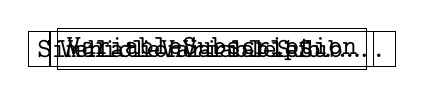
\begin{tikzpicture}
\tikzset{level distance=50pt}
\Tree [.\node[draw]{\texttt{VariableSubscription}};
[.\node[draw]{\texttt{VehicleVariableSub\dots}}; ]
[.\node[draw]{\texttt{SimulationVariableSub\dots}}; ]
[.{\dots} ]
]
\end{tikzpicture}
%    \caption{Árbol de herencia de suscripciones.}
%    \label{fig:subs_tree}
%\end{figure}

\subsubsection{Envío de resultados al cliente}

\texttt{TraCIServer} mantiene una variable de instancia \texttt{tcpip::Storage outgoing}, en la cual se almacenan los mensajes de estado y resultados de comandos TraCI. El envío de estos al cliente se efectúa al final de cada iteración del \emph{loop} en \texttt{waitForCommands()}, enviando así conjuntamente las respuestas a todos los comandos obtenidos desde el cliente en el último paso de tiempo. Gracias a las clases \texttt{tcpip::Storage} y \texttt{tcpip::Socket} utilizadas, la operación de enviar los datos almacenados se reduce a una invocación del método \texttt{sendExact()} del objeto \texttt{tcpip::Socket}, la cual recibe un objeto \texttt{tcpip::Storage}, le adjunta una cabecera con su tamaño total y lo envía a través del \emph{socket} al cliente.

La escritura de datos en el almacenamiento saliente se implementó en dos métodos de \texttt{TraCIServer}; \texttt{writeStatusResponse()}, método de conveniencia para la escritura de mensajes de estado, y \texttt{writeToOutputWithSize()}, el cual recibe otro objeto de tipo \texttt{tcpip::Storage} que contiene el resultado de algún comando y escribe sus contenidos en \texttt{outgoing}, junto con una cabecera que indique su tamaño. Esto implicó también una decisión de diseño en términos de la comunicación de \texttt{TraCIServer} con los demás módulos del sistema. Se optó por realizar la mayor parte de esta comunicación mediante objetos de tipo \texttt{tcpip::Storage}, delegando la estructuración de los resultados de cada comando específico a los módulos responsables. De esta manera se aumenta la modularidad, ya que cada módulo sabe como escribir sus resultados de manera correcta, y \texttt{TraCIServer} sólo necesita asumir que recibirá un \texttt{tcpip::Storage} bien formateado como respuesta a los comandos.

\lstinputlisting[style=CPP, label={code:traciserver_writetooutput},caption={Escritura de datos en almacenamiento saliente.}]{codigo/traciserver_writetooutput.cpp}

\subsection{Simulation}\label{sec:simulation}

La principal funcionalidad de este módulo es controlar el avance de la simulación, además de abstraer y encapsular el acceso a los parámetros de la simulación vehicular de Paramics. Se implementó como una clase de C++ utilizando el patrón de diseño \emph{Singleton}; esto quiere decir que sólo se permite la instanciación de un único objeto de este tipo en la ejecución del programa. Esto ya que, por razones lógicas, cada ejecución del \emph{plugin} está asociada a una única simulación en Paramics, y por ende no tiene sentido que pueda existir más de un objeto de acceso a ésta.

\subsubsection{Avance de la Simulación}

Al recibir un mensaje de avance de simulación, \texttt{TraCIServer} invoca el método \texttt{runSimulation()} del presente módulo, detallado en los anexos, código \ref{code:simstep}. Este método recibe como parámetro un entero representando el instante de tiempo hasta cual se quiere avanzar la simulación (de ser $0$ se interpreta como solicitud de avance de un único paso de simulación) y ejecuta los llamados necesarios a la API de Paramics, además de notificar a \texttt{VehicleManager} que debe actualizar sus listas de vehículos.

\subsection{VehicleManager}\label{sec:vehiclemanager}